\documentclass[10pt]{article}
\usepackage[margin=0.76in]{geometry}
\usepackage[T1]{fontenc}
\usepackage{lmodern}
\usepackage{microtype}
\usepackage{amsmath,amssymb,mathtools}
\usepackage{booktabs,tabularx,array,enumitem}
\usepackage{xcolor,hyperref,fancyhdr}
\usepackage{tikz}
\usetikzlibrary{arrows.meta,positioning,fit}
\hypersetup{
  colorlinks=true,
  hypertexnames=false,
  linkcolor=blue!55!black,
  urlcolor=blue!55!black,
  pdftitle={SCI-ALIGN v0.1 Stage B Targeted Scientific Rationale r0.2},
  pdfauthor={Implementation-blind Stage B author}
}
\definecolor{alignblue}{RGB}{35,91,130}
\definecolor{alignteal}{RGB}{27,122,111}
\definecolor{aligngold}{RGB}{189,124,36}
\definecolor{aligngray}{RGB}{240,243,245}
\setlength{\emergencystretch}{3em}
\setlist{nosep,leftmargin=1.5em}
\newcolumntype{Y}{>{\raggedright\arraybackslash}X}
\newcommand{\code}[1]{\nolinkurl{#1}}
\newcommand{\statusbox}[1]{\par\smallskip\noindent\colorbox{aligngray}{\parbox{0.96\linewidth}{#1}}\par\smallskip}
\pagestyle{fancy}
\fancyhf{}
\fancyhead[L]{SCI-ALIGN v0.1 --- scientific rationale}
\fancyhead[R]{Stage B targeted draft r0.2}
\fancyfoot[C]{\thepage}
\raggedbottom

\title{SCI-ALIGN v0.1\\
\large Scientific Rationale for Sample Identity, Timing Alignment, and Scan Support\\[0.3em]
\normalsize Stage B Targeted Revision r0.2 --- Author Draft}
\author{Implementation-blind Stage B scientific author}
\date{2026-08-22}

\begin{document}
\maketitle

\begin{abstract}
SCI-ALIGN establishes one observation-scoped relation between native detector,
telescope, and admitted auxiliary occurrences and a stable detector-reference
grid.  Its scientific job is narrow but foundational: preserve what happened,
when it happened under an admitted clock relation, how each target slot was
formed, and what support and uncertainty are actually available.  It acts on
the paired raw KID coordinates \(x/r\) only after Tune/readout and before AST,
RTC, calibration, correlated-component treatment, validation policy, or map
deposition.  This narrative explains the scientific logic; the companion
Engineering Conformance Specification retains the complete notation, twenty
canonical equations, fifty-five requirements, and twenty-six predictions.
\end{abstract}

\statusbox{\textbf{Authority status.} This is a Stage B targeted author draft,
not scientific-owner approval.  It does not assess implementation conformity,
observational validation, freeze, operational readiness, or production use.}

\noindent\textbf{Reading guide.} Sections 1--9 follow the scientific questions
in the order a reducer encounters them: identity and time, readout ordering,
field operators, telescope-state ownership, missing support, interval
identity, downstream transfer, and finally response and open decisions.

\vfill
\noindent\textbf{Shared identity rule.} \(s\) is the stable ALIGN
detector-reference slot and \((o,s)\) is its stable observation-scoped
identity.  \(j\) is a local storage row only.  \(n\) is reserved for a stable
RTC output-sample identity.  No downstream contract reconstructs \(s\) from
\(j\).

\clearpage
\section{What ALIGN scientifically establishes}

ALIGN creates a checked, immutable account of temporal relationship.  It does
not make sky coordinates or maps and does not decide whether a later estimator
may use a sample.  It establishes the detector-reference interface
\(i_{\rm ref}=D\), its nominal grid, stable slot identities \((o,s)\), exact
native source relations, field-specific mappings, and local origin, validity,
support, exposure, response, uncertainty-availability, and provenance facts.

The central output is therefore a relation, not merely an array.  A consumer
must be able to distinguish a native occurrence from a nominal slot, an exact
copy from interpolation, a numerical invalidity from a missing occurrence,
and local ALIGN validity from AST validity or named-use eligibility.  Array
shape and row order cannot carry those meanings by themselves.

\section{Native event time versus nominal detector-reference slot}

Each producer owns the event and epoch meaning of its native coordinate.
ALIGN may place an admitted interface on detector-reference time only through
the checked relation
\[
 t^{\rm ref}_{ik}=(E_i-E_{i_{\rm ref}})_{\rm sec}+u_{ik}
 +\delta_{i\rightarrow\rm ref},\qquad
 \delta_{{\rm ref}\rightarrow{\rm ref}}=0.
\]
The offset is observation-constant in v0.1, producer-authorized, expressed in
seconds, and applied exactly once.  The corrected event time remains distinct
from nominal slot time \(t_s\), assignment residual, native integration
support, nominal cell support, and acquired exposure.

\begin{figure}[b]
\centering
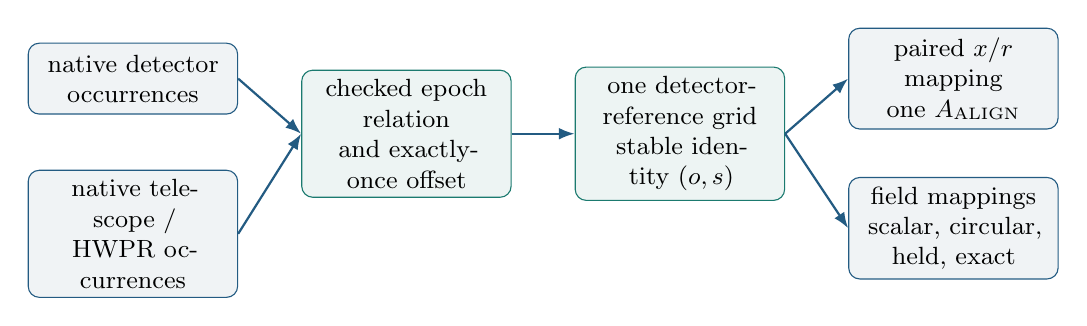
\begin{tikzpicture}[
  node distance=7mm and 8mm,
  box/.style={draw=alignblue,rounded corners,fill=aligngray,align=center,
    minimum height=9mm,text width=0.20\linewidth,font=\small},
  map/.style={draw=alignteal,rounded corners,fill=alignteal!8,align=center,
    minimum height=9mm,text width=0.20\linewidth,font=\small},
  arr/.style={-{Latex[length=2mm]},thick,draw=alignblue}
]
\node[box] (det) {native detector\\occurrences};
\node[box,below=of det] (tel) {native telescope /\\HWPR occurrences};
\node[map,right=of det,yshift=-7mm] (clock) {checked epoch relation\\and exactly-once offset};
\node[map,right=of clock] (grid) {one detector-reference grid\\stable identity $(o,s)$};
\node[box,right=of grid,yshift=7mm] (pair) {paired $x/r$ mapping\\one $A_{\rm ALIGN}$};
\node[box,right=of grid,yshift=-12mm] (fields) {field mappings\\scalar, circular, held, exact};
\draw[arr] (det.east) -- (clock.west);
\draw[arr] (tel.east) -- (clock.west);
\draw[arr] (clock) -- (grid);
\draw[arr] (grid.east) -- (pair.west);
\draw[arr] (grid.east) -- (fields.west);
\end{tikzpicture}
\caption{Native occurrences enter one checked time relation before assignment
to a stable detector-reference grid.  The paired detector coordinates and
each registered field then retain their distinct mapping semantics.}
\label{fig:one-grid}
\end{figure}

\clearpage
\section{Tune/readout before paired \(x/r\) alignment}

The ordinary detector-signal chain is
\[
 (I,Q)^{\rm acq}\longrightarrow\text{Tune/readout}
 \longrightarrow(x,r)^{\rm acq}\longrightarrow\text{ALIGN}
 \longrightarrow(x,r)^A .
\]
Here \(I,Q\) are acquired microwave quadratures, while \(x,r\) are the paired
physical KID readout coordinates.  The symbols \(x\) and \(r\) are reserved
for those coordinates; the detector reference is instead \(i_{\rm ref}=D\).
Tune/readout owns the conversion, its units, normalization, and mapping
revision.  ALIGN neither aligns \(I,Q\) first nor assumes that Tune conversion
commutes with resampling or synthesis.

One realized temporal operator acts separately on both readout coordinates:
\[
 x^A=A_{\rm ALIGN}x^{\rm acq},\qquad
 r^A=A_{\rm ALIGN}r^{\rm acq}.
\]
The outputs share native occurrences, weights, residuals, stable slots,
source-relation identity, and origin/synthesis state.  Numerical validity and
payload availability remain coordinate-specific.  One coordinate never fills
or rescues the other, and no mapping crosses a Tune or readout-revision
boundary without separate authority for that operation, response, and
uncertainty.

This distinction also protects astrometry.  AST can sometimes construct a
coordinate from a valid occurrence/time relation, geometry, and observing
state even when one or both numerical \(x/r\) payloads are invalid or not
requested.  Signal-coordinate validity is transferred, but it is not silently
promoted into AST coordinate validity or downstream eligibility.

\statusbox{\textbf{Nonpolarimetric scope.} ALIGN v0.1 admits only the ordinary
nonpolarimetric detector-signal path.  The \(x/r\) coordinates remain raw KID
readout coordinates.  Optional HWPR timing/alignment facts do not authorize
demodulation, polarization calibration, or Stokes reconstruction.}

\clearpage
\section{Field-specific mapping: scalar, circular, held, and exact-only}

ALIGN does not apply one generic interpolation rule to every telescope or
auxiliary field.  Before mapping, each field needs a versioned registry entry
that fixes identity, unit, source frame, topology, validity and missing-data
meaning, maximum support span, uncertainty availability, and operator.

\begin{center}
\small
\begin{tabularx}{0.95\linewidth}{@{}p{0.18\linewidth}YY@{}}
\toprule
Field class & Permitted mapping & Scientific guardrail \\
\midrule
Continuous scalar & Exact copy at coincidence or bounded adjacent linear
interpolation within one unbroken valid run. & No extrapolation and no
skipping across invalid rows; unit and frame do not change. \\
Circular angle & Exact copy or shortest-arc interpolation using
\(d_P(a,b)\in[-P/2,P/2)\). & Exactly antipodal inputs are unavailable unless
an explicit unwrap authority resolves the path. \\
Declared step state & Hold only inside a producer-authoritative half-open
validity interval. & A held value at a non-native time is synthesized and
retains held provenance. \\
Exact-only & Exact coincidence only. & Between native occurrences the field
is unavailable rather than guessed. \\
\bottomrule
\end{tabularx}
\end{center}

For scalar interpolation at target slot \(s\), the motivating relation is
\[
 y_s=(1-\lambda_s)v_a+\lambda_s v_b,\qquad
 \lambda_s=\frac{t_s-t_a}{t_b-t_a}.
\]
Circular interpolation uses the same fraction but applies it to the declared
shortest signed difference and then wraps into the field's declared period.
The half-open interval is a representation convention, not permission to
choose a path for an exactly antipodal pair.

Timestamp, identity, category, mode, flag, counter, and hardware-state fields
cannot inherit scalar treatment from their numerical representation.  A
missing registry entry blocks only the dependent field or claim and cannot be
recovered from a familiar name, shape, or numerical range.

\clearpage
\section{Observing-state fields versus pointing-correction records}

Two telescope families serve different scientific purposes and must remain
separate.  The observing-state family describes the science occurrence on the
detector-reference grid: aligned boresight, current sample time, current
elevation, required azimuth, and any additional registered values needed by
AST geometry or field rotation.  ALIGN preserves the producer's unit, frame,
topology, support, and meaning.

The pointing-correction family is not another name for current observing
state.  A pointing-support producer selects an exact correction record and its
native support and supplies record, parent, selection, vector-meaning, sign,
basis, unit, time/support, covariance-availability, and producer identities.
ALIGN contributes only the admitted relation of that selected record to
detector-reference time.  AST may interpolate a correction only within the
selected native support and never extrapolates.

In particular, current science-sample elevation is not inferred from a
bracketing correction record.  Field rotation uses the aligned
occurrence-local observing state.  Correction composition, geometry,
continuous sky/map coordinates, astrometric uncertainty, and TAN/WCS
projection remain AST responsibilities.  Physical center selection remains
with the named target or product authority.

Optional HWPR fields are a third typed family.  Their timing and alignment can
be represented without trimming the ordinary nonpolarimetric detector
support.  Until a future polarimetry authority exists, these facts do not
authorize demodulation or Stokes reconstruction.

\clearpage
\section{Original values, interpolation, gaps, continuity surrogates, and exposure}

A nominal grid cell is not evidence that a detector acquired anything.  ALIGN
keeps distinct: a native original occurrence, an interpolated field value, an
acquisition timing gap, an original occurrence with invalid payload, a
processing guard, an unavailable optional stream, and an explicitly
authorized detector-signal continuity surrogate.

Ordinary field interpolation follows the registered operator.  It does not
authorize detector-signal synthesis.  A continuity surrogate would need a
separate signal-domain authority specifying count, duration, fraction, edge,
causal support, response, uncertainty, and guard rules.  That authority is
unresolved in v0.1, so the conditional gap equation in the engineering view
is not enabled.  If ever authorized, a surrogate keeps exact endpoints and
weights, synthesized origin, and zero added acquired exposure; it does not
gain an independent hit, degree of freedom, or significance count.

\begin{figure}[b]
\centering
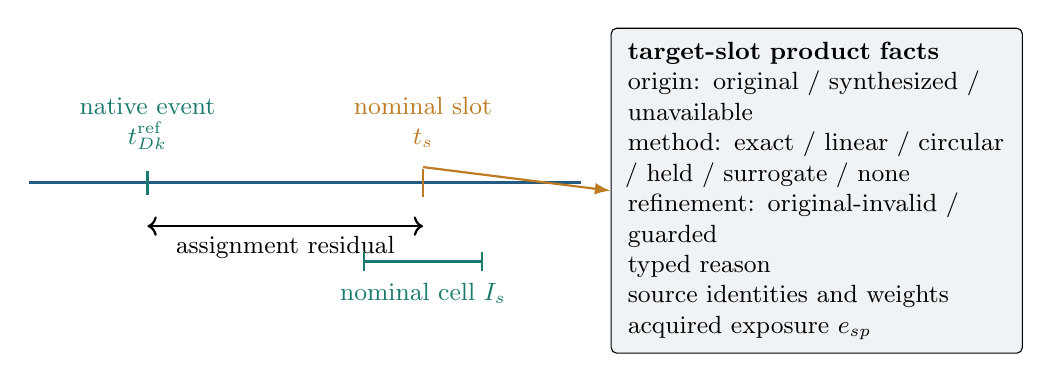
\begin{tikzpicture}[
  arr/.style={-{Latex[length=2mm]},thick},
  lab/.style={font=\small,align=center},
  pill/.style={draw,rounded corners=2pt,fill=aligngray,font=\small,
    align=left,text width=4.8cm,inner xsep=6pt,inner ysep=5pt}
]
\draw[very thick,alignblue] (0,0) -- (7.0,0);
\draw[thick,alignteal] (1.5,-0.15) -- (1.5,0.15)
  node[above=4pt,lab]{native event\\$t^{\rm ref}_{Dk}$};
\draw[thick,aligngold] (5.0,-0.18) -- (5.0,0.18)
  node[above=4pt,lab]{nominal slot\\$t_s$};
\draw[<->,thick] (1.5,-0.55) -- (5.0,-0.55)
  node[midway,below,lab]{assignment residual};
\draw[thick,alignteal] (4.25,-1.0) -- (5.75,-1.0)
  node[midway,below=4pt,lab]{nominal cell $I_s$};
\draw[thick,alignteal] (4.25,-0.88) -- (4.25,-1.12);
\draw[thick,alignteal] (5.75,-0.88) -- (5.75,-1.12);
\node[pill] (facts) at (10.0,-0.1) {\textbf{target-slot product facts}\\
origin: original / synthesized / unavailable\\
method: exact / linear / circular / held / surrogate / none\\
refinement: original-invalid / guarded\\
typed reason\\
source identities and weights\\
acquired exposure $e_{sp}$};
\draw[arr,aligngold] (5.0,0.2) -- (facts.west);
\end{tikzpicture}
\caption{One stable target slot carries distinct timing and product-state
facts.  Origin and support explain how a value exists; acquired exposure
records only attributable native support and is zero for synthesized or
unavailable detector signal.}
\label{fig:slot-anatomy}
\end{figure}

\clearpage
\section{Physical scans versus processing and science windows}

Five interval identities remain separate even when their numerical bounds
happen to coincide:
\begin{enumerate}
\item producer-authoritative physical scan or state interval;
\item processing chunk;
\item science window;
\item context window; and
\item output selection.
\end{enumerate}
Each is stable, observation-scoped, and half-open.  Subsetting or repartitioning
does not renumber physical scans or stable ALIGN slots.  Short, partial, empty,
guarded, and unusable states retain identity rather than being padded away.

A requested fixed-duration partition may define processing windows after its
duration is resolved to a sample count.  It cannot replace physical scan
authority or reinterpret a producer state such as \code{Hold}.  The exact
transition and validity semantics for physical scan segmentation remain an
owner/producer question.

Within a materialized window, local row \(j\) may be derived from stable slot
\(s\) through the explicit selection relation.  That local row is convenient
storage, not external identity.  The stable cross-package key remains
\((o,s)\), while \(n\) remains reserved for RTC output samples.  This rule
prevents a changed slice boundary or array layout from silently changing
scientific identity.

Exposure also follows stable source identity rather than window membership.
Overlapping membership is rejected unless a successor explicitly defines it
and prevents double counting.

\clearpage
\section{What AST and RTC receive}

AST receives one immutable bundle under profile
\code{SCI-ALIGN_TO_SCI-AST v0.1/r0.1}.  The package manifest binds the final
boundary bytes; the boundary body contains no self-hash.  The bundle is not a
menu of substitutable records.  Every required item is present with exact
identity and semantics or typed unavailable with reason.

The transfer includes the reference grid and stable \((o,s)\) identity;
native and assigned timing; offset authority; exact or generatively
reconstructible source relations; the common paired \(x/r\) mapping and
coordinate-specific validity; observing-state and pointing-correction
families; origin, support, exposure, intervals, mapping validity, response,
covariance availability, and complete requested-to-realized provenance.  Each
materialized view carries its explicit \(s\)-to-\(j\) relation.  AST does not
reconstruct clocks, repeat ALIGN policy, extrapolate pointing support, infer
missing semantics, or treat a nominal slot or synthesized value as exposure.

RTC receives stable ALIGN identities and relation facts before owning its own
temporal conditioning and stable output-sample identity \(n\).  CAL owns
calibration and atmosphere operations; PTC owns correlated-component
estimation; VAL evaluates predicates registered by named-use owners; and MAP
owns sample-to-pixel deposition, estimator-specific projection \(G_\pi\),
weights, contribution, and map support.  Every consumer preserves ALIGN
origin, source support, response/covariance availability, and zero exposure
for synthesized detector values.

\statusbox{\textbf{Compatibility rule.} Similar shape or field names do not
establish compatibility.  A successor must name the profile revision it
supersedes and map every changed, removed, or newly required semantic item.}

\clearpage
\section{Response, covariance, validation, and unresolved owner questions}

ALIGN's response is conditional on the realized mapping.  Even a linear
interpolator that preserves DC generally changes amplitude and phase away from
zero frequency.  Gap response, if ever authorized, is row-specific and
nonstationary.  ALIGN therefore exports an exact conditional response for the
admitted tier or a typed reason it is unavailable; it does not claim an
end-to-end downstream transfer function.

When a full admitted joint covariance is supplied, an affine realized mapping
uses \(C_{y\mid A}=A C_{v\mid A}A^{\mathsf T}\), preserving known cross-time,
cross-detector, and cross-stream terms.  Timing, interpolation-model, mapping,
and selection uncertainties are reported when admitted or typed unavailable,
never silently set to zero.  Shared interpolation endpoints do not create
independent information.

The engineering predictions define future falsifiable comparisons, not
validation evidence.  No named implementation, data product, observing run,
or executable path was assessed in this targeted revision.

\subsection*{Compact rationale-to-contract crosswalk}
\begin{center}
\small
\begin{tabularx}{0.95\linewidth}{@{}p{0.30\linewidth}Y@{}}
\toprule
Narrative topic & Engineering authority \\
\midrule
Identity, checked time, grid & EQ-001--003; REQ-002--015; PRED-001, 002, 009 \\
Paired \(x/r\) relation & EQ-006--007; REQ-001, 004--006; PRED-019--021 \\
Field operators and telescope families & EQ-004--005; REQ-016--023; PRED-005, 006, 022, 025 \\
Gaps, origin, exposure, intervals & EQ-008--010, 018--020; REQ-024--036; PRED-007, 008, 010, 014, 026 \\
Transfer, response, covariance & EQ-011--017; REQ-037--055; PRED-004, 012, 013, 023, 024 \\
\bottomrule
\end{tabularx}
\end{center}

\subsection*{Owner decision register summary}
Open or deferred decisions remain: producer event/epoch and offset domains
(ODQ-101); exact observing-state registry (102); physical scan/\code{Hold}
semantics (103); detector continuity-surrogate policy (104); response,
covariance, and detail tiers (105); exact HWPR registry and all polarization
science (109); and exact pointing-correction registry (110).  Decisions
106--108 remain closed as recorded.  Each unresolved item blocks only its
dependent field, operation, or claim.

\statusbox{\textbf{Final status.} This targeted draft records scientific
semantics for owner review.  Implementation conformity, validation, scientific
approval, freeze, readiness, and production authorization remain unassessed.}

\end{document}
